\documentclass[a4j,11pt]{jarticle}
\usepackage{fancyheadings,listings}
%\usepackage{here}
\lstset{
  basicstyle={\ttfamily},
  identifierstyle={\small},
  commentstyle={\smallitshape},
  keywordstyle={\small\bfseries},
  ndkeywordstyle={\small},
  stringstyle={\small\ttfamily},
  frame={tb},
  breaklines=true,
  columns=[l]{fullflexible},
  numbers=left,
  xrightmargin=0zw,
  xleftmargin=3zw,
  numberstyle={\scriptsize},
  stepnumber=1,
  numbersep=1zw,
  lineskip=-0.5ex
}
\setlength{\headheight}{15.5pt}
\usepackage[dvipdfmx]{graphicx, color}
\renewcommand{\thepage}{\small -- \arabic{page} --}
%\headrulewidth=0pt
\rhead{}
\lhead{}
\textheight 234mm
%
\usepackage{amsmath}	% required for `\cases' (yatex added)
\usepackage{bm}
\usepackage{ascmac}	% required for `\screen' (yatex added)

\newcommand{\thisyear}{2019}

\pagestyle{fancy}
\lhead{2025$BG/EY(B $B%W%m%0%i%_%s%0(BIII}

\title{2025$BG/EY(B $B%W%m%0%i%_%s%0(BIII $BBh(B1$B2s(B $B%l%]!<%H(B}
\date{2025 $BG/(B10$B7n(B2$BF|(B}

\author{学籍番号36714029 \\ 遠藤裕人}
%
%
\begin{document}
%
\maketitle
\clearpage
%
%
\section{$B$O$8$a$K(B}
%
%
$B1i=,2]Bj(B1$B$N<B9T7k2L$K$D$$$FJs9p$7$^$9!#(B
%
%
\section{$B1i=,2]Bj(B}
%
%
\subsection{2.1 課題3-1}
この出力結果のように
a=2.5のとき出力は2.500000000となる \\
b=2.5のとき出力は2となる\\

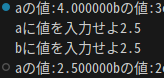
\includegraphics[height=30mm, width=30mm]{task3-1-output.png}

\subsection{2.2 課題3-2}

\begin{lstlisting}[caption=hoge. label=fuge]
  #include<stdio.h>
  int main(void)
  {
      int height;
      float weight; 
  
      printf("身長を入力せよ");
      scanf( "%d", &height);
      weight = (height - 100) * 0.9;
  
      printf("標準体重は%.1fです", weight);
  }
\end{lstlisting}
出力:\\
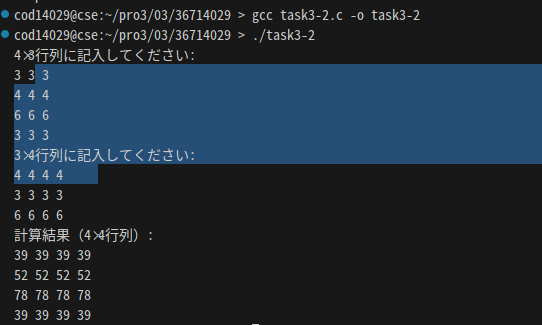
\includegraphics[height=30mm, width=30mm]{task3-2-output.png}

\subsection{2.3 課題3-3}

\begin{lstlisting}[caption=hoge. label=fuge]
  typedef struct {
    //生徒id
    int id;
    //科目の点数
    int subject[2];
} student;

int main(void) {
    // 構造体の利用例
    student s[4] = { {1, {80, 90}}, {2, {85, 95}}, {3, {78, 88}}, {4, {30, 69}} }; // 2番目の生徒を選択

    int total_subject1 = 0;
    int total_subject2 = 0;
    for(int i = 0; i < 4; i++) {
        total_subject1 += s[i].subject[0];
        total_subject2 += s[i].subject[1];
    }
    printf("一科目目の合計点 %d, 二科目目の合計点: %d\n", total_subject1, total_subject2);
    printf("一科目目の平均点 %d, 二科目目の平均点: %d\n", total_subject1/4, total_subject2/4);
    
    int total_student1 = s[0].subject[0] + s[0].subject[1];
    int total_student2 = s[1].subject[0] + s[1].subject[1];
    int total_student3 = s[2].subject[0] + s[2].subject[1];
    int total_student4 = s[3].subject[0] + s[3].subject[1];
    for(int i = 0; i < 4; i++) {
        printf("%d番目の生徒の合計点 %d\n", i+1, s[i].subject[0] + s[i].subject[1]);
    }
    for(int i = 0; i < 4; i++) {
        printf("%d番目の生徒の平均点 %d\n", i+1, (s[i].subject[0] + s[i].subject[1])/2);
    }
}
\end{lstlisting}
出力:\\
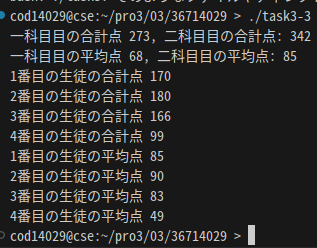
\includegraphics[height=30mm, width=30mm]{task3-3-output.png}

$B<BAu7k2L(B
$B3X@RHV9f(B: 36714029 $B;aL>!'!!1sF#!!M5?M(B
\end{document}
